\documentclass[9pt,a4paper,twocolumn]{article}
\usepackage[margin=0.9in]{geometry}
\usepackage{hyperref}
\usepackage[final]{pdfpages}
\usepackage{subcaption}
\usepackage{cite}
\usepackage[acronym]{glossaries}

 \setlength{\columnsep}{0.25in}

\makeglossaries

\newacronym{scc}{SCC}{Strongly Connected Components}

\title{An Analysis of the Portuguese Section of Wikipedia}

\author{Daniel Ramos \\ 81620 \and Miguel Tavares \\ 83528 \and Ricardo Brancas  \\ 83557}

\begin{document}
\maketitle

\section{Introduction}
The goal of this project is to analyse and characterise a real world network, and to  get acquainted with tools and methods which will be useful in following endeavours.
As such, we have chosen to analyse a snapshot of the Portuguese section of Wikipedia \cite{dataset};
we have chosen such a large network in order to get familiarised with Webgraph \cite{webgraph}.

%TODO

To analyse our data we use Webgraph, including snippets of code made available
by Prof. Alexandre Francisco \cite{aplf}.

\section{Methods}
The network was originally represented as an edge list which was subsequently converted in an adjacency list (ASCII Graph), by use of a simple \texttt{C++} program, as this is the input
format for Webgraph's compression algorithms.

After running Webgraph, we used a Python script to parse the output and generate the figures present in this document.


\section{Results and Discussion}

The network we have chosen contains $1\,603\,222$ vertices and $49\,021\,409$ edges. Both the minimum in and out-degrees are $0$, the maximum in-degree is $207\,254$ while the maximum out-degree is $12\,237$, finally the combined average degree is approximately $61.15$. Furthermore, there are 121 \acrlong{scc}, the largest being comprised of $1\,602\,960$ nodes.
\vspace{1\baselineskip}

\begin{figure}[h]
	\centering
	\begin{subfigure}{.475\textwidth}
		\centering
		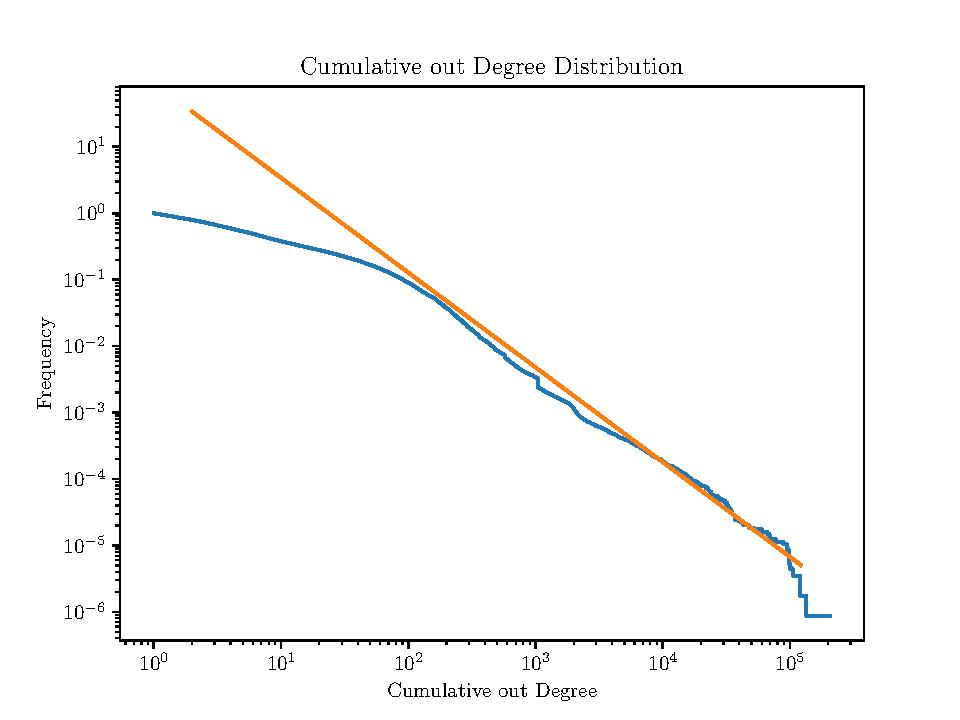
\includegraphics[width=\linewidth]{wikipedia_pt_in.pdf}
		\caption{Cumulative in-degree distribution.}
		\label{fig:inddist}
	\end{subfigure}
	\begin{subfigure}{.475\textwidth}
		\centering
		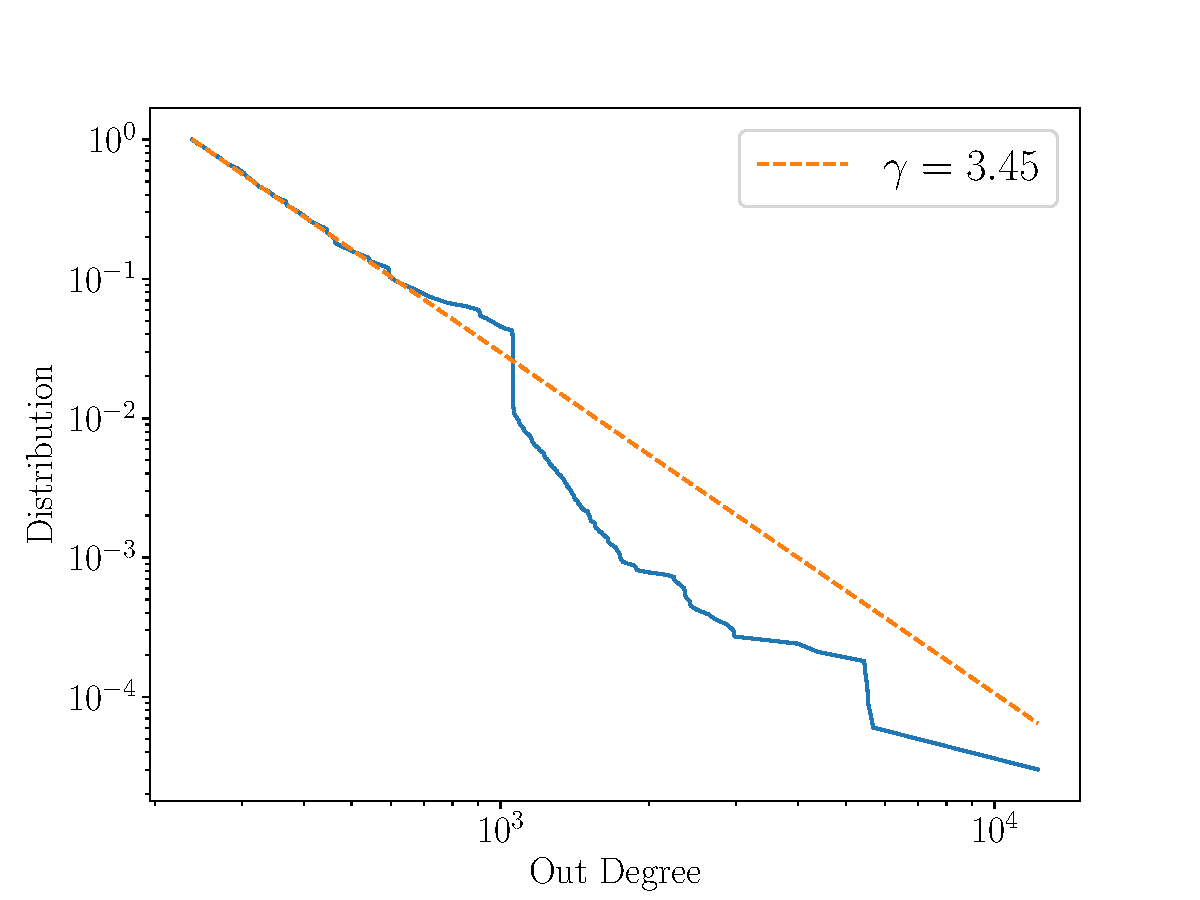
\includegraphics[width=\linewidth]{wikipedia_pt_out.pdf}
		\caption{Cumulative out-degree distribution.}
		\label{fig:outddist}
	\end{subfigure}
	\caption{Degree distributions.}
\end{figure}

In figures ~\ref{fig:inddist} and~\ref{fig:outddist} we present the cumulative in-degree distribution and out-degree distribution, respectively, and their power law regressions. The regressions were obtained using NumPy through a simplified method based on the one described by Clauset et al. \cite{Clauset2009}.

We have found that our degree distributions correlate highly with a power-law distribution, excluding the effects of low degree saturation and high degree cutoff; expected results of the finite nature of real networks.

Based on the regressions computed, we found an in-degree parameter $\gamma = 2.42$ that is lower than its out-degree counterpart $\gamma = 3.89$. This difference in parameters helps explain the disparity between the maximum out-degree and the maximum in-degree. Although our data is unlabelled, we believe this phenomenon occurs because there are few Wikipedia pages which reference most of the others (ie. indexes), leading to a higher $\gamma$ in the out-degree distribution. Conversely, the in-degree distribution parameter $\gamma~=~2.42$ is lower because pages are comparatively more uniformly referenced. %TODO THIS IS WRONG

The variance for the in-degree distribution is $206\,082.30$. This result is also expected as the power-law distribution has a $\gamma = 2.42$ implying a divergent variance for an infinite set. The variance of the out-degree distribution is significantly lower at $6\,296.66$, which is also expected, since a $ \gamma = 3.89 $ implies a finite variance, hence the lower value.

\begin{figure}[h]
	\centering
	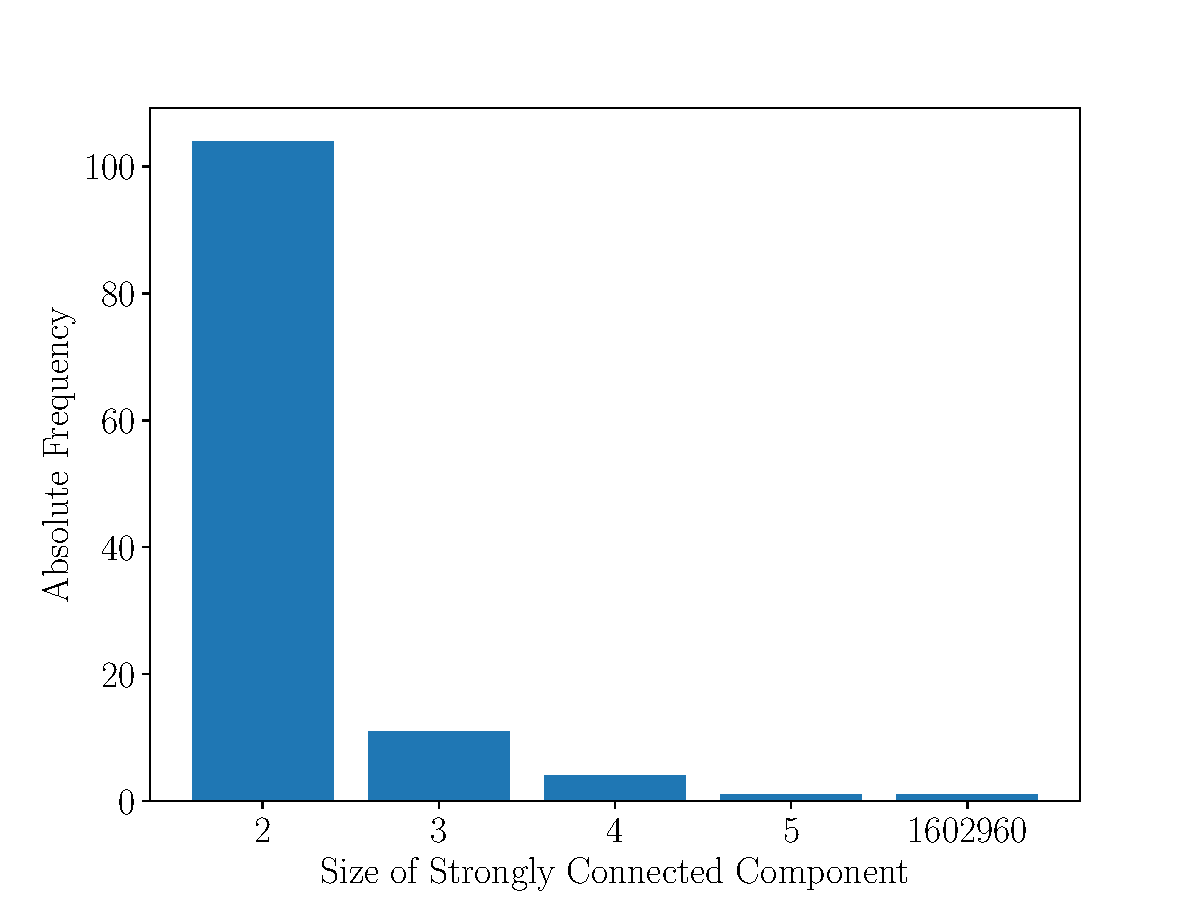
\includegraphics[width=\linewidth]{wikipedia_pt_sccdistr.pdf}
	\caption{Strongly Connected Component distribution.}
	\label{fig:sccdist}
\end{figure}

Figure \ref{fig:sccdist} shows the number of \acrshort{scc}s in respect to their cardinality. We notice a giant strongly connected component, as expected, containing almost all the nodes ($1\,602\,960$) in the graph, and also a very few small ones. These results are in accordance with the expected results if the network were a random graph as the average degrees obtained ($> ln(N)$) imply a connected regime.

However our graph is not connected, and as such it is impossible to compute the diameter through the usual method. Thus we used the effective diameter, a more robust measure that calculates the diameter using $90\%$ as a cut-off of the cumulative probability function. We obtained an effective diameter of $5.8361 \pm 0.0022$. An alternative and even more significant measure is the Harmonic Diameter, which we learned to be $6.8982 \pm 0.0403$.
Considering, again, that the network were a random graph, the expected Average Path Lenght would be $\frac{ln(n)}{ln(k)} = 4.2$, which is not too far from the obtained value.

\begin{figure}[h]
	\centering
	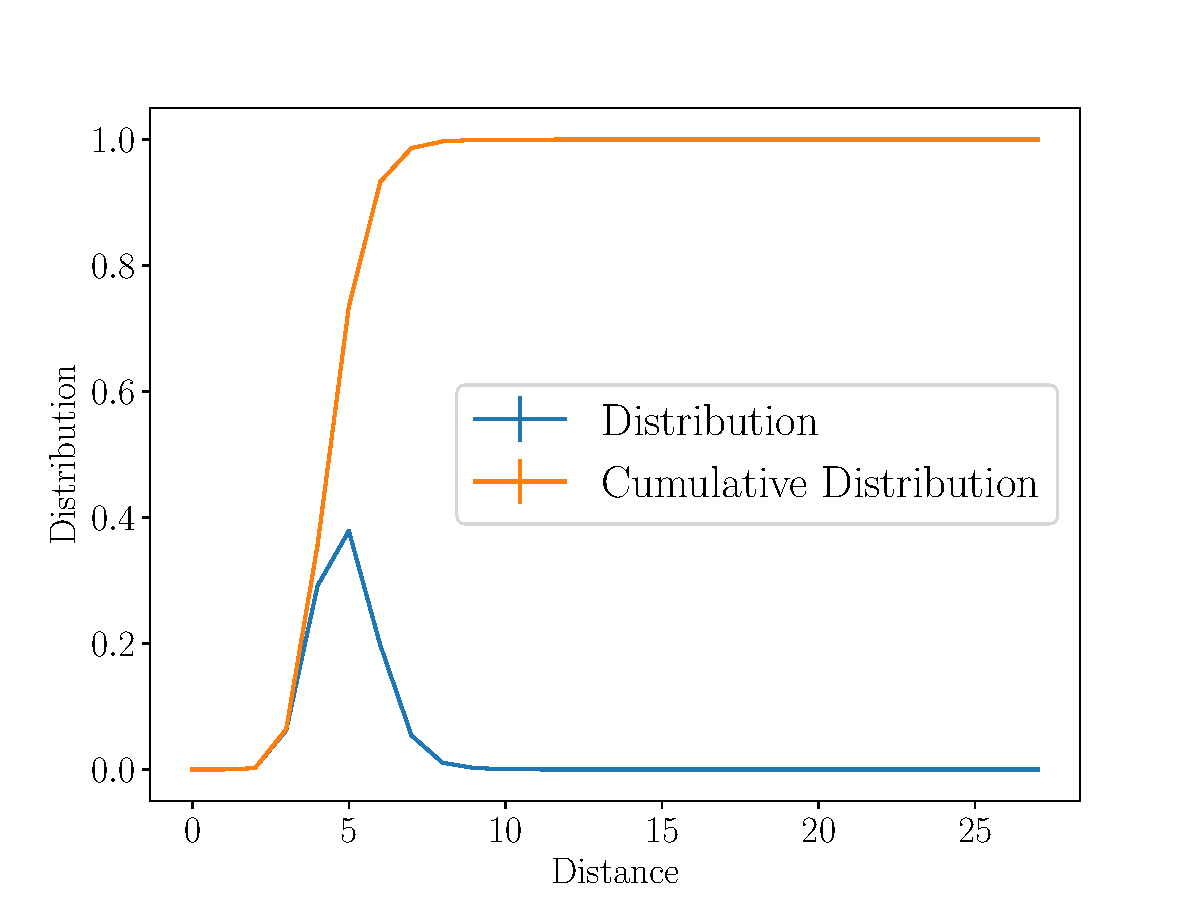
\includegraphics[width=\linewidth]{wikipedia_pt_neighbourhood_function.pdf}
	\caption{Approximate neighbourhood function.}
	\label{fig:neighfun}
\end{figure}

In figure \ref{fig:neighfun} is we present the Approximate Neighbourhood Function computed by Webgraph and averaged through JackKnife. This measure represents for each $t \in N$, the number of pairs of nodes $ \langle x, y \rangle $ such that $y$ is reachable from $x$ in less than $t$ hops \cite{Boldi2011HyperANFAT}.

We have also obtained an estimation of the Average Path Length through HyperBall \cite{DBLP:conf/icdm/BoldiV13}. The estimated value is $ 4.9290 \pm 0.0026 $. This result is in accordance with the values observed in Figure~\ref{fig:neighfun}: roughly a half of the nodes can be reached from each other in just 5 hops. As such, we conclude the Portuguese Wikipedia page's to have approximately 5 degrees of separation, on average.

\begin{figure}[h]
	\centering
	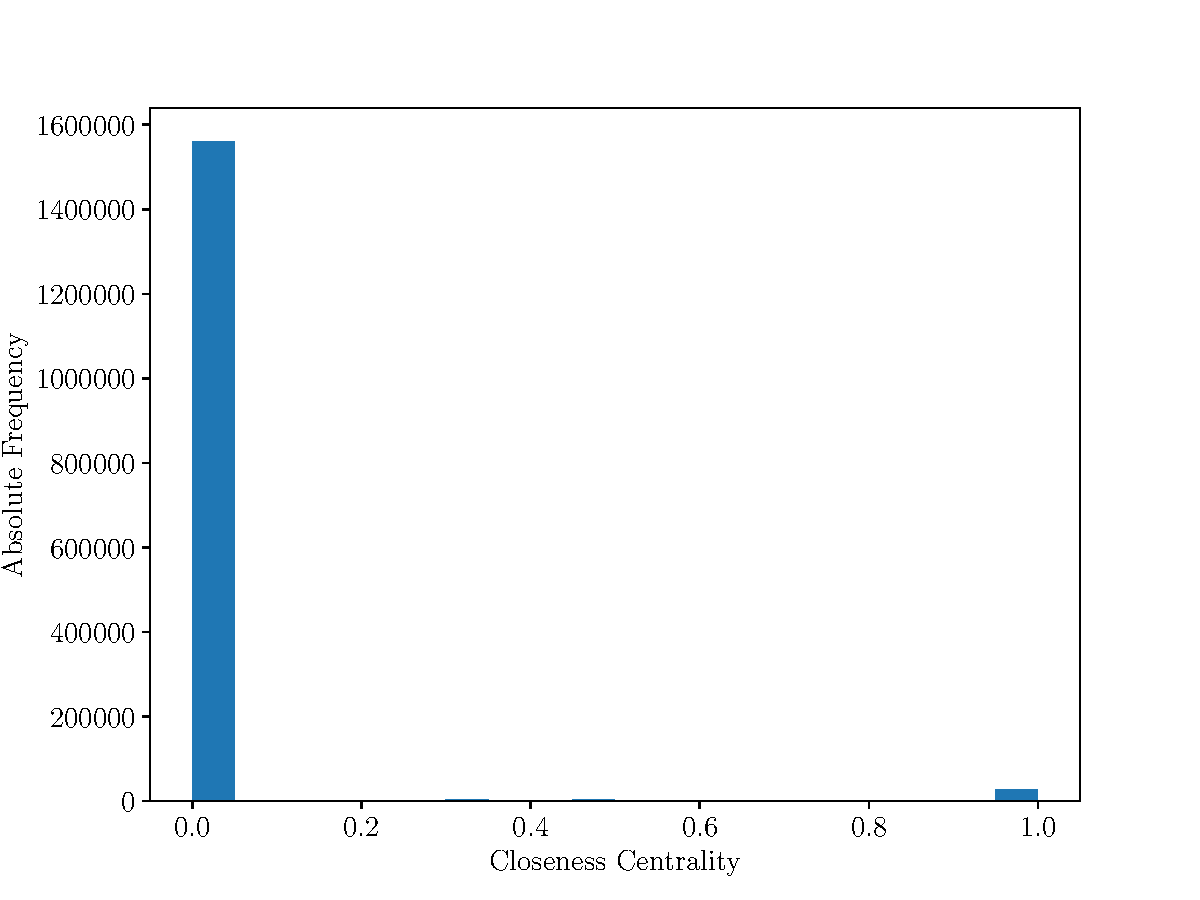
\includegraphics[width=\linewidth]{wikipedia_pt_closeness_centrality.pdf}
	\caption{Closeness centrality.}
	\label{fig:closeness}
\end{figure}

\begin{figure}[h]
	\centering
	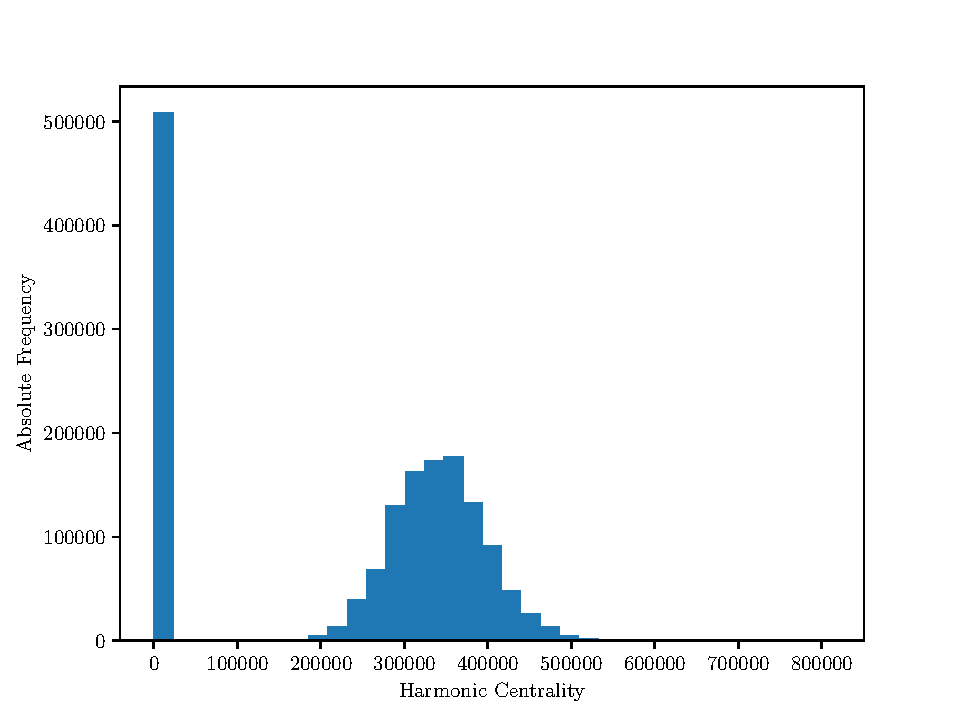
\includegraphics[width=\linewidth]{wikipedia_pt_harmonic_centrality.pdf}
	\caption{Harmonic centrality.}
	\label{fig:harmonic}
\end{figure}

Out of curiosity we decided to estimate the closeness centrality, and the results are just as expected. As it can be seen in Figure~\ref{fig:closeness} almost all nodes have a closeness centrality of 0, this is due to our graph not being connected. Since this measure does not give us any further information on the graph, we also decided to calculate the harmonic centrality, which nicely allows the existence of disconnected nodes by giving them less weight than to the closer vertices, which means their contribution is close to 0. Figure~\ref{fig:harmonic} exhibits the obtained results.

We have also verified a Shortest Path Index of Dispersion (SPID) of $0.2287 \pm 1.9232 \times 10^{-4}$, which according to Boldi et al. \cite{Boldi2011HyperANFAT} correlates to a ``properly social" network.

\section{Conclusion}

In short we conclude that the Portuguese section of Wikipedia displays a scale free behaviour, governed by a power law distribution. The regression gammas, as is usual in Web networks, are higher for the out-degree distribution than for the in-degree.


escrever coisas sobre o maximum out e in degree serem muito diferentes

\printglossary[type=\acronymtype]

\bibliographystyle{plain}
\bibliography{references}

\end{document}
